% !TEX root = ./Basilisk-navAggregate-2019-02-21.tex

\begin{figure}[htb]
	\centerline{
	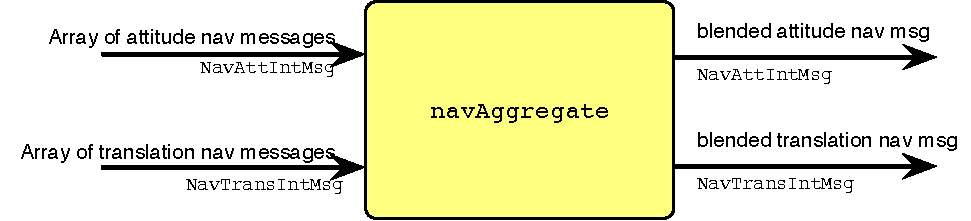
\includegraphics[]{Figures/moduleImg}
	}
	\caption{Illustration of the {\tt navAggregrate()} input and output messages.}
	\label{fig:moduleImg}
\end{figure}

\section{Module Description}
The purpose of this simple aggregate module is to read in a series of navigation messages, and combine their values into a single output message.  The module is able to blend both attitude and translation navigation messages.   

The number of input messages is defined through either {\tt attMsgCount} or {\tt transMsgCount}.  If either of these values is zero, then the corresponding output navigation message is populated with zero components.  

To select which input message value to use, the module index value must be set for that particular parameter.  All these variables end with {\tt Idx}.  Their default values are 0, indicating that by default the values of the first navigation message are used.   By changing the {\tt Idx} value the user selects which message content to use for that variable.  This can be set individually for each navigation message variable.   If the {\tt Idx} value is larger than the number of input messages, then the corresponding variable is set to zero values.  This allows the output message to zero out particular variables.  In all cases the {\tt Idx} index must be less than input navigation message counter  {\tt attMsgCount} or {\tt transMsgCount} respectively.  
